\section{Experiments}\label{sec:experiments}
\vspace{-2mm}

In this section, we thoroughly evaluate \method{} both in simulation and in real.
%
% investigate the impact of our design choices to train \method{}, ranging from simulation to real world. 
%
We train \method{} in a simulated version of Unitree G1 using IsaacLab~\citep{MittalYYLRHYSGMMBSHG23} at 200 Hz, while the control frequency is 50 Hz. For the behavior dataset, we use the LAFAN1 dataset~\citep{HarveyYNP20lafan1} retargeted to the Unitree G1 robot. The LAFAN1 dataset contains $40$ several-minute-long motions. 
%For training, we utilize all the motions, but we split them into chunks of $10$ seconds to achieve a more fine-grained selection for motion prioritization during training. %We also interpolate motions in DOF space to match the control frequency.
We also demonstrate generality of \method{} on a Booster T1 humanoid (App.~\ref{sec:t1-sim}).

%This section demonstrates the experimental validation of our framework using both simulations and real-world deployment on the Unitree G1 humanoid robot, highlighting its ability to produce diverse and robust behaviors when prompted with different tasks (e.g., motion tracking, reward and goal-reaching).

% \textbf{Motion datasets.} For the behavior dataset we use the LAFAN1 dataset~\citep{HarveyYNP20lafan1} retargeted to the Unitree G1 robot. The LAFAN1 dataset contains $40$ several-minute-long motions. For training, we use all the motions but we split them into chunks of $10$ seconds to have a more fine-grained selection for motion prioritization in training. We also interpolate motions in DOF space to match the control frequency. 

% \textbf{Simulation environments.} For sim-to-sim evaluation, we use a similar Unitree G1 model but simulated with DeepMind MuJoCo~\citep{TodorovET12}. 
% We tried to match the two simulators as closely as possible in terms of physical parameters, but some differences are unavoidable even in the DR implementation.

% \textbf{Downstream tasks and metrics.}
% We evaluate the model's performance in three main categories of downstream tasks:
% % \begin{itemize}[noitemsep,topsep=0pt,parsep=0pt,partopsep=0pt,leftmargin=0.5cm]
% % \item 
% \textit{(1) Reward optimization}: This category includes reward functions designed to test a variety of behaviors. Performance is measured by the average return over episodes lasting 500 steps. 
% % \item 
% %\item
% \textit{(2) Motion tracking}: This category tests the model's ability to replicate a target motion beginning from its initial pose. Similar to previous work~\citep{Luo2023phc,Chen2025gmt}, we report the average joint 3D Cartesian position error $E_{\mathrm{mpjpe}}$, averaged over the whole motion.
% For testing, we consider motions in the training LAFAN1 dataset as well as $175$ out-of-distribution motions from the CMU subset of the AMASS motion-capture dataset~\citep{Mahmood2019AMASS}.
% \textit{(3) Pose reaching}: This category evaluates the model's ability to reach a specified goal starting from arbitrary initial conditions and to stay as close as possible, even when poses may not be easy to stabilize. We consider $21$ manually selected poses from motions in the LAFAN1 dataset and report the error $E_{\mathrm{mpjpe}}$, averaged over the whole rollout of $500$ steps (10 seconds). For OOD evaluation we further extract 10 poses from the motions in the AMASS dataset.
% \end{itemize}

% \begin{figure}[t]
% \centering
% \begin{minipage}[t]{.3\textwidth}
%     \centering
%     \tiny
%     \begin{tabular}{@{}lccc@{}}
%         \toprule
%         \textbf{Model} & \multicolumn{3}{c}{\textbf{Sim-no-DR}} \\
%         \cmidrule(lr){2-4}
%          & Track & Rwd & Pose \\
%         \midrule
%         \textsc{BFM-oracle} &  &  &  \\
%         \textsc{BFM-noDR}   &  &  &  \\
%         \bottomrule
%     \end{tabular}
% \end{minipage}
% \hspace{0.01\textwidth}
% \begin{minipage}[t]{.6\textwidth}
%     \centering
%     \tiny
%     \begin{tabular}{@{}lccccc@{}}
%         \toprule
%         \textbf{Test} & \multicolumn{2}{c}{\textbf{Track}} & \textbf{Rwd} & \multicolumn{2}{c}{\textbf{Pose}} \\
%         \cmidrule(lr){2-3} \cmidrule(lr){5-6}
%          & LAFAN1 & AMASS &  & LAFAN1 & AMASS \\
%         \midrule
%         Sim-DR         & $+1.1\%$ (0.013) & $-1.3\%$ (0.030) & TODO & $+7.9\%$ (0.035) & $-6.5\%$ (0.020) \\
%         Sim-to-sim-DR  & $+0.6\%$ (0.009) & $+0.0\%$ (0.025) & TODO & $+25.3\%$ (0.039) & $+77.5\%$ (0.028) \\
%         \bottomrule
%     \end{tabular}
% \end{minipage}
% \caption{Tracking, reward, and pose-reaching performance across models for different testing configurations. numbers in () represents cv. 
% \textcolor{red}{what is CV?}
% }
% \label{fig:tracking_results}
% \end{figure}


% \begin{figure}[t]
% % \begin{table}[t]
%  \centering
%  \begin{minipage}[t]{.38\textwidth}
%     \resizebox{.99\textwidth}{!}{%
%     \begin{tabular}{|c||c|c|c|}
%         \hline
%     Model & \multicolumn{3}{|c|}{Sim-no-DR}\\
%         \hline
%         \hline
%         & Track & Rwd & Pose  \\
%         \hline
%         \textsc{BFM-Zero-oracle} & & & \\
%         \textsc{BFM-Zero-noDR} & & & \\
%         \hline
%     \end{tabular}
%     }
% % \end{table}
% \end{minipage}
%  \begin{minipage}[t]{.61\textwidth}
% % \begin{table}[t]
%  \centering
%     \resizebox{.99\textwidth}{!}{%
%     \begin{tabular}{|c||c|c|c|c|c|}
%         \hline
%     Test & \multicolumn{5}{c|}{\textsc{BFM-Zero}}\\
%         \hline
%         \hline
%         &\multicolumn{2}{c|}{Track} & Rwd & \multicolumn{2}{c|}{Pose}\\
%         & LAFAN1 & AMASS &  & LAFAN1 & AMASS \\
%         \hline
%         %Sim-DR & & & & & \\
%         %Sim-to-sim-DR & & & & & \\
%         Sim-DR & $+1.1\%$ cv=$0.013$ & $-1.3\%$ cv=$0.030$ & TODO & $+7.9\%$ cv=$0.035$ & $-6.5\%$ cv=$0.020$ \\
% Sim-to-sim-DR & $+0.6\%$ cv=$0.009$ & $+0.0\%$ cv=$0.025$ & TODO & $+25.3\%$ cv=$0.039$ & $+77.5\%$ cv=$0.028$ \\
%         \hline
%     \end{tabular}
%     }
% % \end{table}
% \end{minipage}
% \caption{Tracking, reward, and pose-reaching performance across models for different testing configurations.}
% \end{figure}

% \begin{figure}[t]
% \centering
% % \includegraphics[width=.9\textwidht]{}
% \caption{Normalized distribution for tracking, reward and pose-reaching performance. For each task (i.e., motion, reward, pose), we compute the normalized score w.r.t.\ the range of \textsc{BFM-Zero-noDR} and plot the distribution. \matteo{(x - range(noDR).min())/range(DR-nohist)}}
% \end{figure}

% \begin{table}[]
%     \centering
%     \scriptsize
%     \resizebox{.99\textwidth}{!}{%
%     \begin{tabular}{lccc ccc ccc}
%         \toprule
%         \textbf{Model} & \multicolumn{3}{c}{\textbf{Sim-no-DR}} 
%                        & \multicolumn{3}{c}{\textbf{Sim-DR}} 
%                        & \multicolumn{3}{c}{\textbf{Sim-to-sim-DR}} \\
%         \cmidrule(lr){2-4} \cmidrule(lr){5-7} \cmidrule(lr){8-10}
%          & Track & Rwd & Pose & Track & Rwd & Pose & Track & Rwd & Pose \\
%         \midrule
%         \textsc{FB-CPR-oracle} & 1.0749 & 299.3 & 1.0291 &      &       &       &       &       &       \\
%         \textsc{FB-CPR-noDR}   & 1.0909 & 278.5 & 1.1123 & 1.1655 & 216.9 & 1.1766 &       &       &       \\
%         \textsc{FB-CPR-hist}   &        &       &        & 1.1015 & 221.9 & 1.1387 & 1.0789 & 207.3 & 1.1041 \\
%         \bottomrule
%     \end{tabular}}
%     \caption{Tracking, reward, and pose-reaching performance across models for different testing configurations. 
%     We only report combinations that are meaningful for the tests described in Sect.~\ref{ssec:sim.experiments}. 
%     One metric per task category is reported: EMD for tracking and success for pose. 
%     \ale{To review once we decide what metrics to include.} 
%     \anssi{Example data for now. MJPJE. 95th percentile over motions (track, goal), then mean.} 
%     \guanya{change the name to \method{}}}
%     \label{tab:sim.experiments}
% \end{table}

\begin{figure}
\begin{minipage}[t]{.4\textwidth}
    %\begin{table}[]
        \scriptsize
    \setlength{\tabcolsep}{4pt}
    \renewcommand{\arraystretch}{1.5}
    \begin{tabular}{llllll}
    \toprule 
    \textbf{Model}      & \textbf{Test env.}   & \textbf{Test data}   & \textbf{Track} & \textbf{Rwd} & \textbf{Pose} \\
    \midrule 
    \method{}-\emph{priv} & Isaac (no DR) & LAFAN1 & 1.0749 & 299.3 & 1.0291 \\
    \method{} & Isaac (DR) & LAFAN1 & 1.1015 & 221.9 & 1.1387 \\
    \method{} & Mujoco (DR) & LAFAN1 & 1.0789 & \multirow{2}{*}{207.3} & 1.1041  \\
    \method{} & Mujoco (DR) & AMASS & 1.0342 &  & 1.4735  \\
    \bottomrule
    \end{tabular}
    %\end{table}
\end{minipage}
\hspace{0.2\textwidth}
\begin{minipage}[]{.3\textwidth}
\centering
    %\begin{figure}[t]
    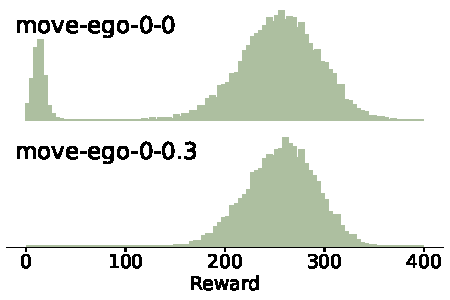
\includegraphics[width=.94\textwidth]{image/reward_hist_two_tasks_hist_simdr.pdf}
    %\end{figure}
\end{minipage}
\caption{\small Tracking, reward, and goal-reaching performance across models for different testing configurations (left), and example distributions of reward evaluation scores for \method{} in Isaac (DR) (right). Each metric is averaged over tasks. We consider the average return over episodes lasting 500 steps for reward, the average joint position error $E_{\mathrm{mpjpe}}$ averaged over the whole motion for tracking, and the error $E_{\mathrm{mpjpe}}$ averaged over the episode for goal-reaching.}
        \label{tab:sim.experiments}
\end{figure}


\subsection{Zero-shot Validation in Simulation}\label{ssec:sim.experiments}
\vspace{-3mm}
In this section, we quantitatively assess the performance and robustness of \method{} along different dimensions in simulation.

\textbf{Asymmetric learning and domain randomization.} We consider a \emph{privileged} version of \method{} where all components of the algorithm receive privileged information. We train this model in a simulated environment with nominal dynamical parameters (\emph{No DR}), and we test it in the very same configuration. This serves as an idealized configuration similar to the problems where unsupervised RL was previously shown to work~\citep{TirinzoniTFGKXL25zeroshot}, although it leads to a model that is \emph{not deployable} on the real robot. We then compare to \method{} trained and tested on a domain randomized version of the environment (\emph{Sim DR}), which corresponds to the model actually deployed on the real robot. Overall, \method{} is $2.47\%$, $25.86\%$, $10.65\%$ worse than \method{}-priv across tracking, reward, and pose reaching tasks. This shows that despite the algorithmic changes made in \method{} compared to FB-CPR, the learning dynamics is still correct and the model retains a satisfactory performance compared to its idealized version. Interestingly, reward tasks suffer from a larger drop in performance. This is in part due to the sparse nature of the reward functions we consider, which makes them less forgiving to suboptimal behaviors and amplify any model error. We also conjecture that this may be related to the reward inference process with domain randomized data. In Fig.~\ref{tab:sim.experiments} we also show the distribution of the performance of \method{} for two representative reward functions across repetitions of the inference process\footnote{In the reward inference, we use a dataset of states randomly subsampled from the training dataset. As a result, multiple repetitions of the process may return different policies.} and episodes. While for \texttt{move-ego-0.3} the performance is fairly consistent, for \texttt{move-ego-0.0}, we notice that a few instances obtained very poor performance. We conjecture that this is related to the increased randomness of the data observed during training due to domain randomization, which makes inference with a small subsampled dataset more brittle and prone to failure.


\textbf{Sim-to-sim performance.} We evaluate the robustness of \method{} to the dynamics of the humanoid by testing it in Mujoco. We notice that performance difference is limited (i.e., all variations are less than $7\%$), showing that the domain randomization at training and the history components in the actor and critics contribute to a good level of robustness and adaptivity.

\textbf{Out-of-distribution tasks.} Finally, we evaluate \method{} on a different set of tracking and pose reaching tasks obtained from the AMASS dataset~\citep{Mahmood2019AMASS}. We consider $175$ out-of-distribution motions from the CMU subset of the AMASS and $10$ manually-selected poses from the motions in the entire AMASS dataset. We run tests in Mujoco to combine different dynamics and out-of-distribution tasks. While a direct comparison of performance between LAFAN1 and AMASS tasks may be misleading due to the specific nature of the motions and poses used in the evaluation, we notice that overall \method{} is able to successfully generalize and complete tracking and pose reaching even when exposed to tasks that are not represented in the training data.

% \textbf{Test 1: What is the performance gap due to asymmetric learning?} 
% We want to investigate the impact of asymmetric learning in our unsupervised RL training where the space of rewards implicitly learned through $B$ and the regularized policy learning now leverage different information. We train a full privileged information model (\textsc{FB-CPR-oracle}) and compare it with one where the policy uses a history $s^h_t$ (\textsc{FB-CPR}). We train and test both models on the same simulation configuration with no form of domain randomization. \ale{Conjectured result is that the gap is ``small'' across all metrics.} \yitang{maybe also training curves}
% While asymmetric learning is an established approach for standard reward-based RL in robotics and partially-observable environments in general, no prior investigation is available on its impact in unsupervised RL and in particular in a complex algorithm FB-CPR, where the space of rewards implicitly learned through $B$ and the regularized policy learning now leverage different information. In order to assess the impact of asymmetric learning on the overall performance, we train a full privileged information model (\textsc{FB-CPR-oracle}) and compare it with one where the policy uses a history $s^h_t$ (\textsc{FB-CPR}). We train and test both models on the same simulation configuration with no form of domain randomization. \ale{Conjectured result is that the gap is ``small'' across all metrics.}

% \textbf{Test 2: Is domain randomization needed?} A typical approach to mitigate the sim-to-real gap is to train policies under perturbations both in the observation and in the simulator's dynamics in order to produce more robust behaviors. We assess the level of robustness of the learned policies by training \textsc{FB-CPR} with or without domain randomization, while then testing on the same environment but with domain randomization. We further test the trained models in a sim-to-sim scenario, where the underlying testing simulator is different from the training one. \ale{Conjectured result is that training without DR would perform very poorly when tested on an environment with DR both in sim and sim2sim.}

% \textbf{Test 3: Are models trained with domain randomization sufficiently robust?} While the previous tests show that history-dependent policies have a small gap w.r.t.\ learning with privileged information and domain randomization leads to behaviors that are more robust, the overall model is not capable of adaptation to the actual dynamics of the testing environment. We then train \textsc{FB-CPR-hist}, where all architectures use a history $s^h_t$. This gives to the critics, which already have access to the privileged state, the capability of adapting to non-observable aspects of the environment dynamics. \ale{Conjectured result is that the hist model works better than standard one and it has smaller variance across DR as it can better adapt to the specific dynamics instance in each episode.} \yitang{I think we can just compare model-vanila v.s. model+history+dr (dont need to separate dr and hist)}



% We consider 6 training configurations: asymmetric training, policy using privileged information and fully unprivileged (all models use only proprioceptive information), with and without domain randomization. These variations are used in the ablation studies to assess the impact of each component on the final performance. The only model test on the real-robot is the one with asymmetric training and domain randomization. The model without domain randomization was not safe to deploy on the real robot.



% \subsection{Sim-to-sim Validation}
% In simulation we ablate the impact of domain randomization and of the asymmetric training, we do not ablate the auxiliary reward since this is specifically designed for sim-to-real. To access whether there is a drop in performance due to the asymmetric training, as mentioned above, we train an oracle model (non-deployable) where the actor also uses privileged information. To assess the performance of the trained domain randomization across various environments, we create validation environments with different levels of domain randomization. We report the different configurations of domain randomization in Table~\ref{tab:domain_rand}. Furthermore, we evaluate the impact of domain randomization by testing the model in a sim-to-sim scenario where we evaluate the model on a simulated environment in DeepMind MuJoCo~\citep{TodorovET12}.

% \begin{table}[t]
%     \centering
%     \begin{tabular}{}
%     \end{tabular}
% \end{table}

% \textit{Downstream tasks and metrics.}
% The formal evaluation consists of three main categories:
% \begin{itemize}
% \item Reward Optimization: This category includes XXX reward functions designed to encourage a variety of behaviors. Performance is measured by the average return over episodes lasting 500 steps. 
% \item Goal Reaching: This category evaluates the model's ability to reach a specified goal starting from arbitrary initial conditions. We consider XXX manually selected ``stable'' poses. Two metrics are used: success rate, which measures whether the goal position is reached at any time, and proximity, which is the normalized average distance to the goal over time.
% \item Tracking: This category tests the model's ability to replicate a target motion beginning from its initial pose. A motion is deemed successfully tracked if the agent stays within a defined threshold of joint position and rotation distance from the target motion throughout its duration, as described in~\citep{LuoHYK21}. Additionally, the earth mover's distance~\citep[][EMD]{RubnerTG00} is used as a less-restrictive metric that does not require perfect time-alignment between the agent's trajectory and the target motion.
% \end{itemize}
% We furthermore present qualitative results showcasing the model's ability to perform motion in-betweeness, stitching and blending.

% We report the results of the ablation studies in Table~\ref{tab:sim2sim_results}. We summarize the main findings below.


% \paragraph{No performance loss due to asymmetric training.} {\color{red} Placeholder for results showing no significant drop in performance due to asymmetric training but loss if we use only proprioceptive information for training}

% \paragraph{No performance loss due to penalties.} {Penalties were a big thing we had to fight against. Should we demonstrate that we can recover the original performance with enough training?}

% \paragraph{Larger model performs better but requires more regularization.} {Larger models reached better metrics (and reached better results), but we had to penalize/dr them more. Maybe experiments to show this? E.g., non-penalized medium model > non-penalized residual model in sim2sim, but when penalized, the result is flipped?}

% \paragraph{Domain randomization improves robustness.} {\color{red} Placeholder for results showing that only the model trained with domain randomization perfoms well across all the DR configurations and simulators.}

% \paragraph{Sim-to-sim correlation with sim-to-real.} {Should we have a section on usefulness of sim2sim results for indicating what could work in sim2real? This is not actually helping our sim2real work at this point (too late), but as an insight this would be useful (e.g., how to setup the sim2sim in a way that reflects accurattely how the robot will work, and what things to track)}

% \paragraph{Qualitative evaluation.} {\color{red} Placeholder for qualitative results.}
% \vspace{-3pt}
\subsection{Zero-shot Validation on the Real Robot}

Finally, we deploy the \method{} model zero-shot on a real Unitree G1 robot. In real-world validation, we aim to \textbf{1)} qualitatively confirm the model's tracking, reward optimization, and goal reaching capabilities on a few selected tasks; \textbf{2)} assess its robustness to perturbations and failures (e.g., falling). \emph{All results in this section come from \textbf{one} model.}

% \ale{Explain more in detail the things we show in the videos}


%
\begin{figure}[t]
    \centering
    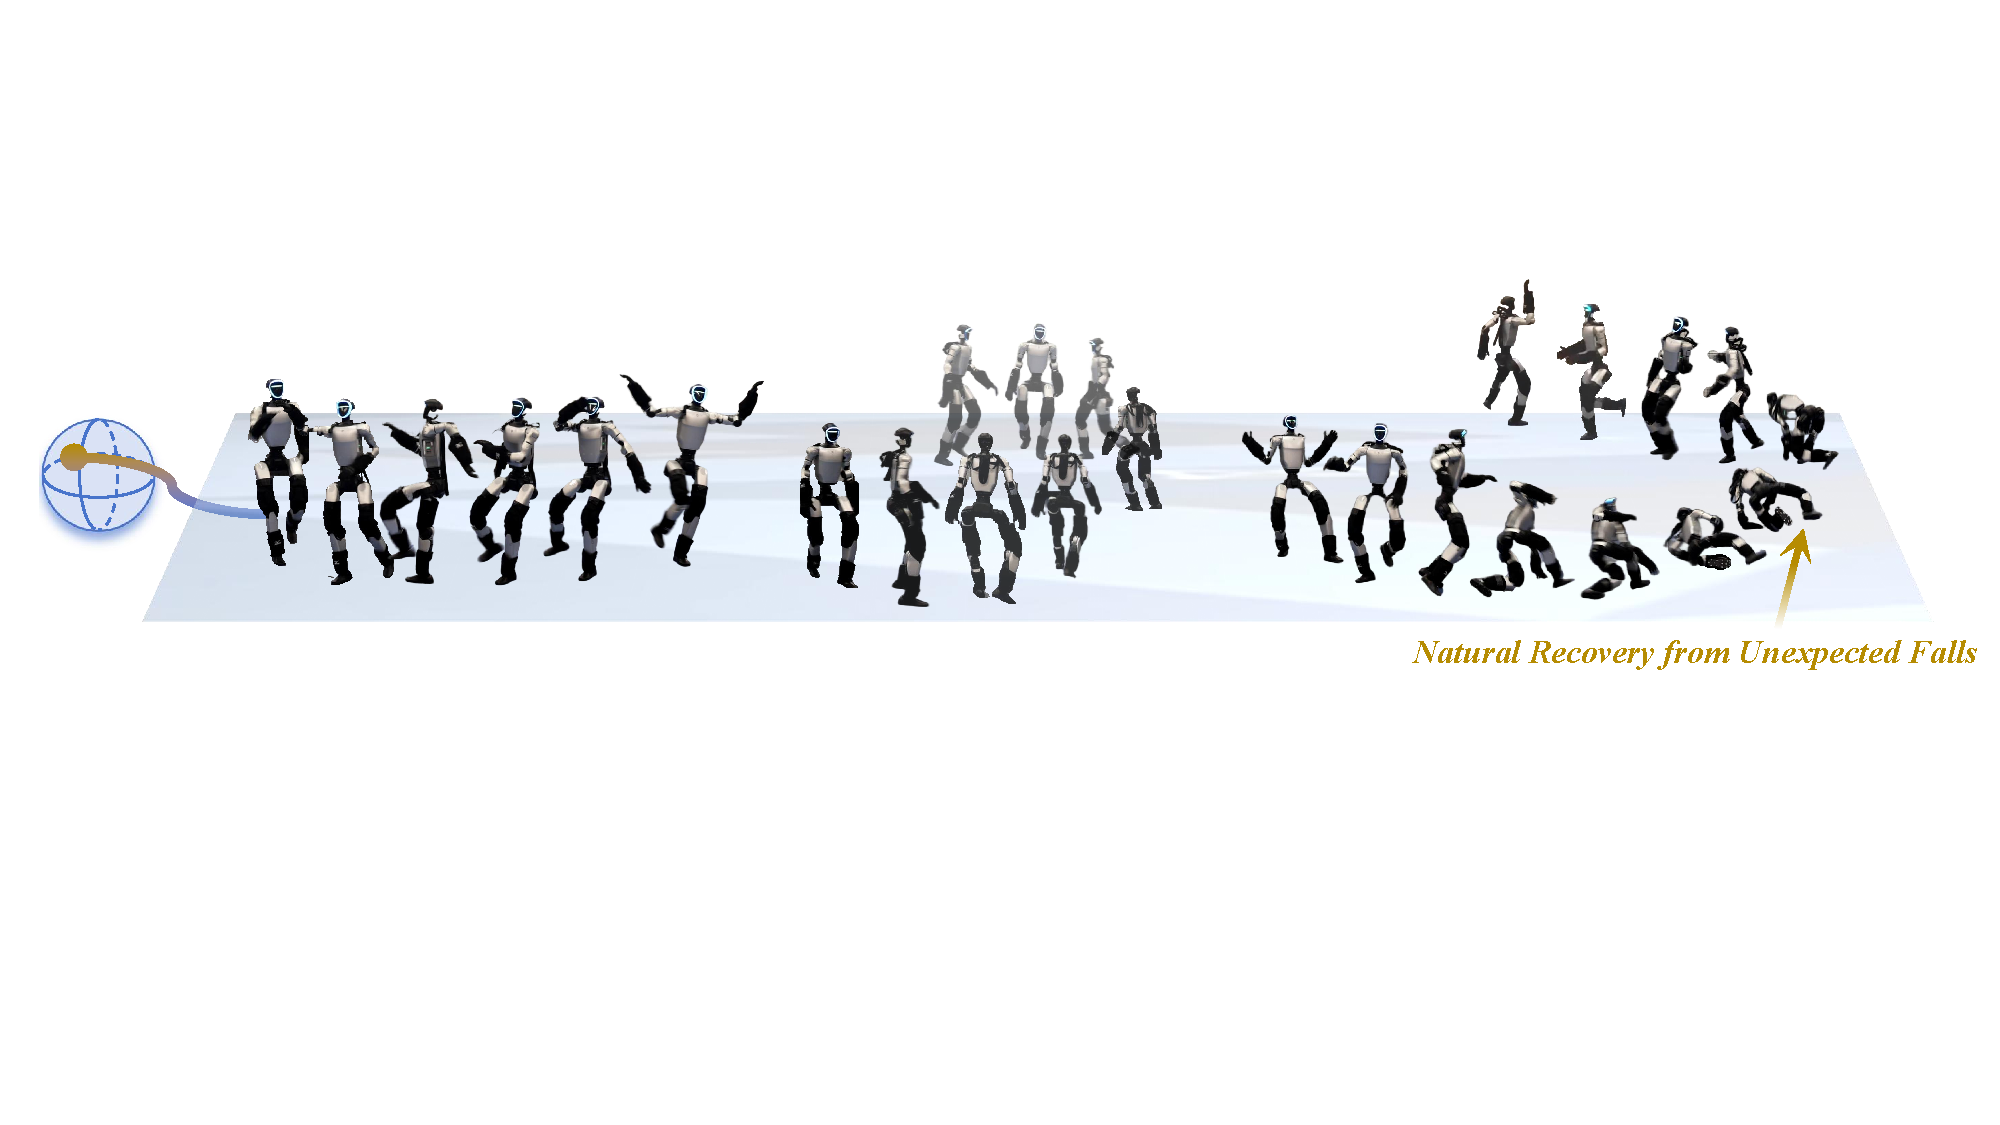
\includegraphics[width=\linewidth]{image/tracking_inference_1.pdf}
    \caption{Real-World Validation of \textbf{Tracking}. \emph{Left:} Highly dynamic dancing. \emph{Middle:} Frequently turning during walking. \emph{Right:} \textbf{Naturally} recover to continue track the motion.}
    \label{fig:tracking_inference}
\end{figure}
%
% it can track diverse motions, including xxxxx 
% it can track low quality ood motions in lalaland (even the motion is with some non continuous states)
% even not stable (falling down), it shows a very gental and natural behaviors during getting up, and keep tracking. not just robustness by trained with lots of disturbance, but truly have a human-like skill library by exposed to lots of motions that make it use some of the skills to continuously complete tracking 
% 
%
\textbf{Tracking.}
As shown in Fig.~\ref{figure_1_teaser} and Fig.~\ref{fig:tracking_inference}, \method{} enables the robot to track various motions, including styled walking motions, highly dynamic dances, fighting and sports. Even when becoming unstable or during a fall (\emph{Right}), it demonstrates remarkably gentle, natural, and safe behavior while recovering and continues tracking seamlessly. This capability stems not merely from robustness gained through disturbance training, but mostly from \emph{TD-based off-policy training} and the use of a GAN-based reward which explicitly encourages human-likeness and regularization terms that enable it to draw upon a rich skill library—much like a human—to adapt and complete tracking seamlessly. 
%
% the exposure to a wide range of human-like motions, enabling it to draw upon a rich skill library—much like a human—to adaptively complete the tracking task. 
%
% As shown in Figure~\ref{figure_1_teaser}, \ref{fig:tracking_inference}, \method{} enables robot to track diverse motions, including various walking styles, highly dynamic dances, fighting, and sports. Even when unstable or falling (\emph{Right}), it demonstrates remarkably gentle, natural, and safe behavior while recovering and continues tracking seamlessly. This capability stems not merely from robustness gained through extensive disturbance training, but from exposure to a wide range of human-like motions, enabling it to draw upon a rich skill library—much like a human—to adaptively complete the tracking task. 
%
Additionally, to evaluate the coverage and generalization capability, we used real videos and retargeted them to the G1.
%robot using~\citep{shen2024gvhmr,alhafez2023b}. 
Despite the suboptimal motion quality and discontinuities introduced by occlusions of monocular videos and artifacts in video estimation, the system is robust to lower quality data and can still successfully track these motions.

% As shown in Figure\ref{fig:tracking_inference}, our model can continuously track diverse motion within a single policy, including various walking styles, highly dynamic dances, fighting, and sports. 

% To test generalization, we evaluate out-of-distribution motions from AMASS and retargeted sequences from online sources. Even when mocap data is corrupted or low quality—producing fragmented trajectories—the model still tracks them effectively. In challenging motions where balance is lost, the robot can safely and naturally get up and resume tracking. This shows that our policy, with tracking-inference z, effectively handles out-of-tracking-state observations and produces natural recovery skills.

\textbf{Goal Reaching.}
%
\begin{figure}[t]
    \centering
    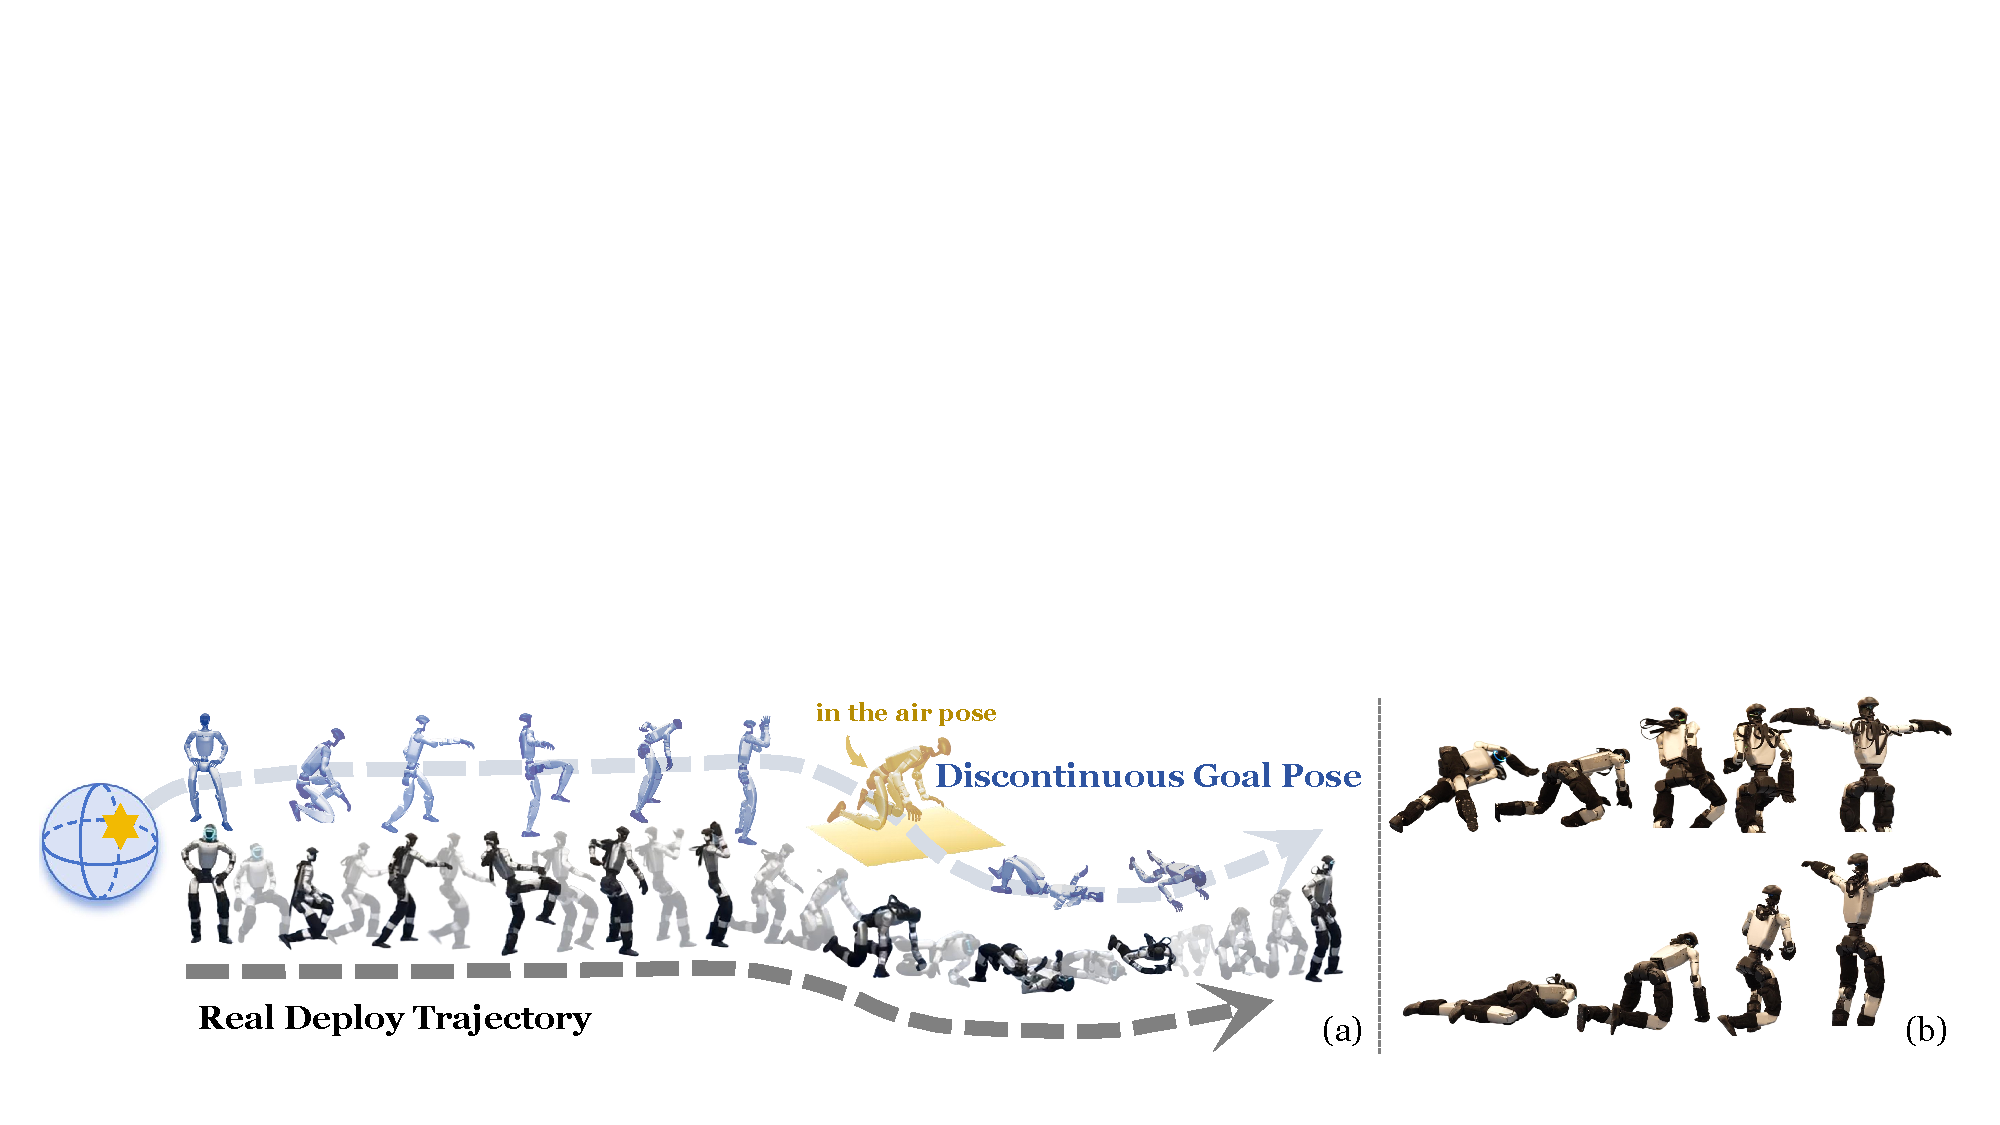
\includegraphics[width=\linewidth]{image/goal_reaching_final_1.pdf}
    \caption{\small Real-World Validation of \textbf{Goal Reaching}. (a) Continuously goal-reaching: the blue/yellow pose denotes the goal pose, while black marks the real robot pose, and gray visualizes the transition between each pose. (b) Transition from any pose to T-pose.}
    \label{fig:goal_inference}
\end{figure}
%
For the goal-reaching task, we extract a sequence of target poses by randomly sampling the goal states and discarding their velocity components. The zero-shot latent of these poses are then permuted and sequentially provided to the policy. As illustrated in Fig.~\ref{fig:goal_inference}, the robot consistently converges to a natural configuration that closely approximates the target pose, even when the target is infeasible (the Yellow one in Fig.~\ref{fig:goal_inference}). Moreover, the resulting trajectory exhibits smooth and natural transitions without the need for explicit interpolation, whether between successive and discontinuous targets(Fig.~\ref{fig:goal_inference}.a) or from an arbitrary pose to the T-pose(Fig.~\ref{fig:goal_inference}.b), demonstrating the smoothness of the learned skill space. 

% For the goal-inference task, we synthesize a sequence of target pose by randomly sampling goal states and discarding their velocity components. We can derive the latent for these quasi-static poses, permuted and presented to the policy in an arbitrary order. Figure~\ref{fig:goal_inference} demonstrates that the robot consistently converges to a natural configuration that approximates the—potentially infeasible—target. Furthermore, the trajectory exhibits smooth, natual between successive targets without requiring auxiliary interpolation schemes, thereby corroborating the implicit regularization conferred by the BFM latent manifold.

% For goal inference, we randomly generate some goal state with velocity values removed as target pose, and shuffle them in a sequence and sequentially reach them. As shown in Figure~\ref{fig:goal_inference}, the policy is able to reach a natural final pose close to the target, even when the target pose is not physically feasible. Moreover, without any explicit interpolation, it transitions smoothly from one pose to another, further highlighting the strong regularization properties of the BFM space.



\begin{figure}[t]
    \centering
    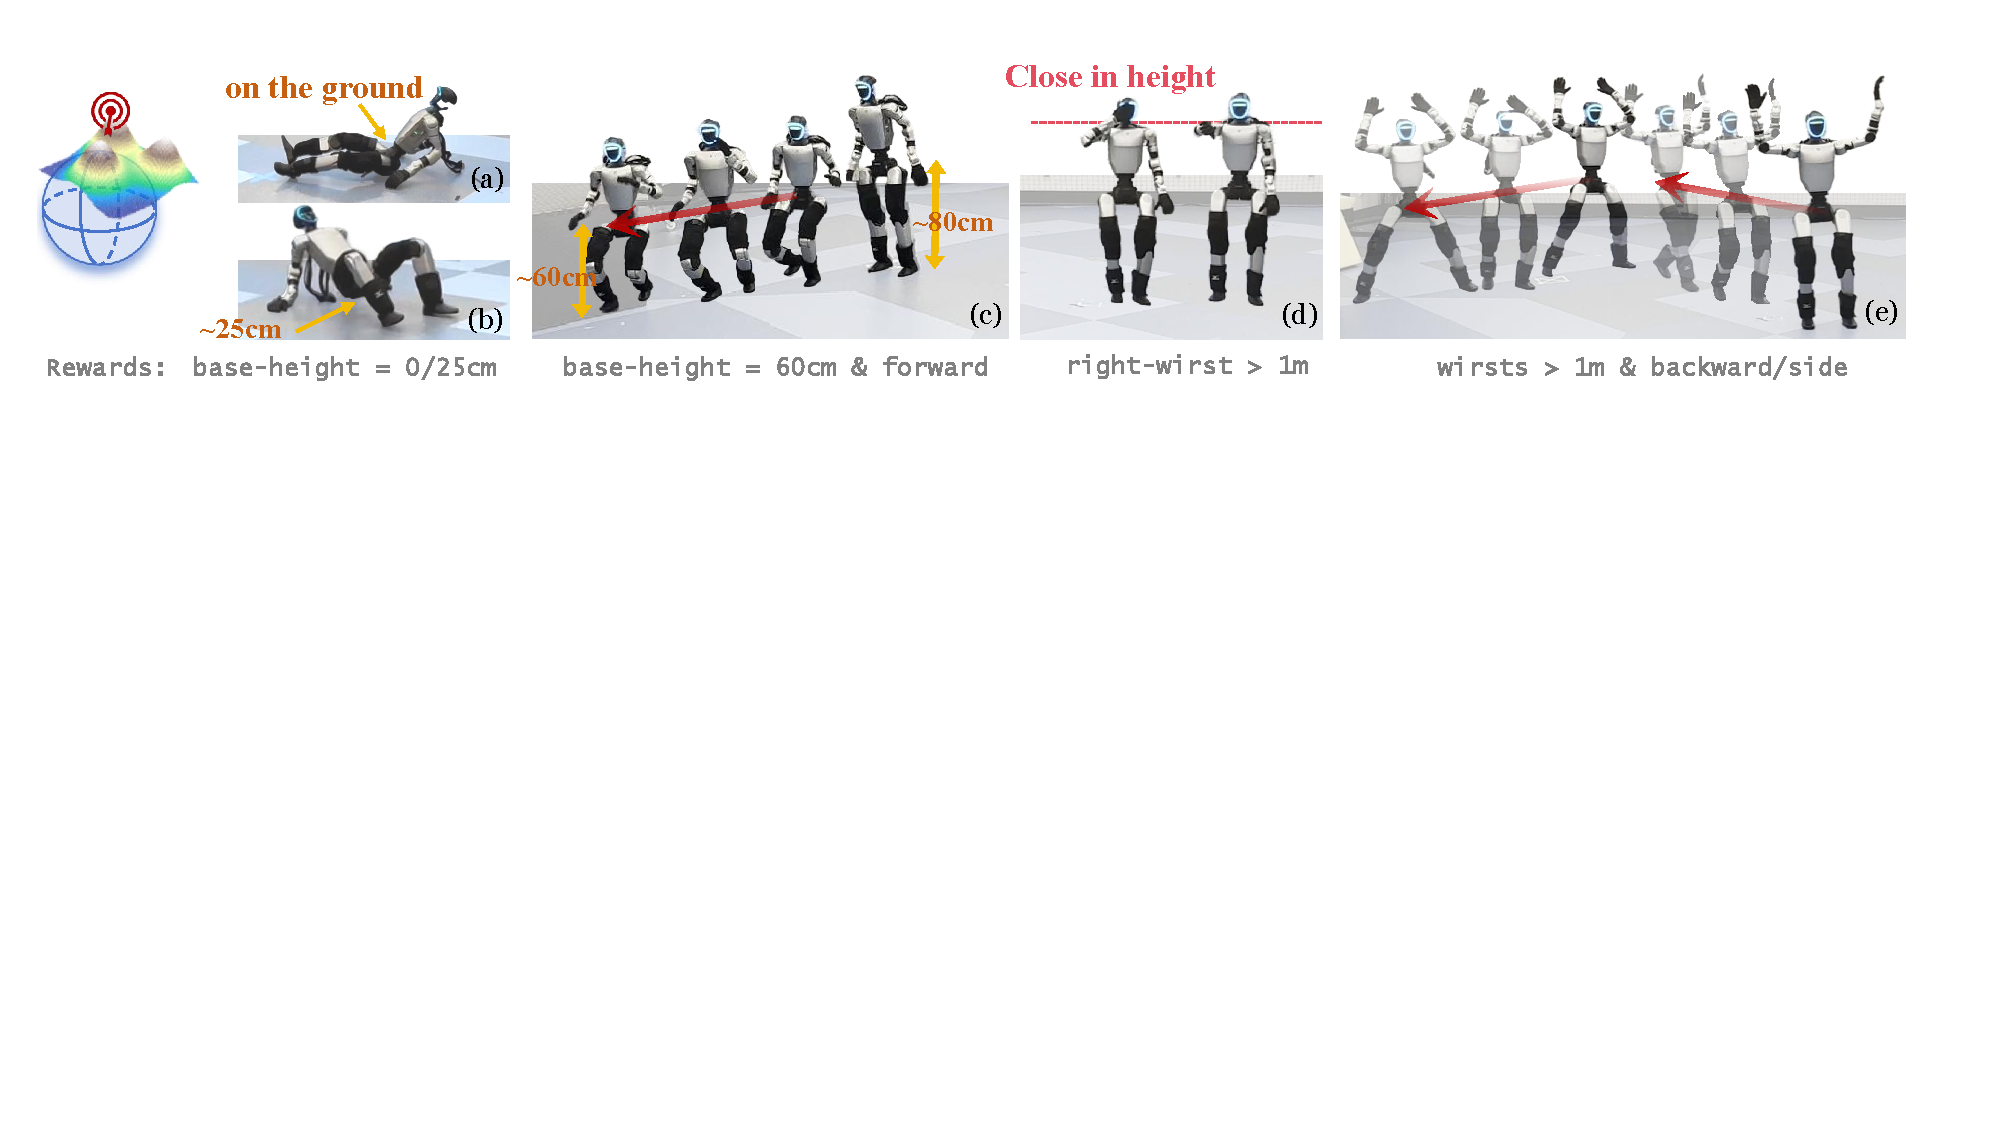
\includegraphics[width=\linewidth]{image/reward_optimization_final.pdf}
    \caption{\small Real-World \textbf{Reward Optimization}. The red arrow represents the base velocity tracking target. (a) \texttt{sitting}; (b) \texttt{crouch-0.25}; (c) \texttt{move-low0.6-ego-0-0.7}; (d) Diverse behaviors from \emph{one} reward \texttt{raisearm-m-l}; (e) combing \texttt{raisearm-m-l} with \texttt{move-ego-180-0.3} and \texttt{move-ego--90-0.7.}}
    \label{fig:reward_inference}
\end{figure}

% We evaluate reward inference in the real world with \emph{locomotion rewards} (moving and rotating, as shown in Figure~\ref{figure_1_teaser}), \emph{arm movement rewards}, and \emph{pelvis height control rewards} (sitting, crouching, or moving at low height, as shown in Figure~\ref{fig:reward_inference} (a,b,c)). All reward functions are defined in Appendix~\ref{app:rewards}. Even with simple reward definitions, the robot faithfully executes base-height, base-velocity, and arm-motion commands. Furthermore, we can get a combination of skills by simply combining rewards, enabling skill-level scaling and the emergence of novel behaviors.
% Also, testing the top-k latents instead of a weighted average reveals multiple behavior modes for loosely defined reward objectives(shown in Figure \ref{fig:reward_inference}(d)). With reward as objective formulation, our policy is friendly to language prompts and intuitive for human use.

% A single policy performs zero-shot inference across these diverse skills using reward-centric commands that are promptable and intuitive for human use. Testing the top-k latents instead of a weighted average reveals multiple behavior modes for loosely defined reward objectives. Moreover, by combining reward terms, the policy composes new skills on the fly, enabling skill-level scaling and the emergence of novel behaviors.
\textbf{Reward Optimization.}
We evaluate reward optimization in the real world with three task families: (i) locomotion rewards that specify base velocities and angular velocities, (ii) arm-movement rewards that command wrist height, and (iii) pelvis-height rewards that request sitting, crouching, or low-movement (Fig.~\ref{fig:reward_inference}(a–c)); reward definitions in Appendix~\ref{app:rewards}.
With simple reward definitions, the robot faithfully executes base-height, base-velocity, and arm-movement commands. Composite skills can be derived from simply linear combination of the rewards (e.g. going backward while raising arms), demonstrating controllable skill-level interpolability. Also, given a specific reward, averaging over different mini-batches from the replay buffer yields a set of latent variables that represents a diverse collection of potential optimal modes as shown in Fig.~\ref{fig:reward_inference}(d). Formulating objectives through reward functions makes our policy intuitive for human users and receptive to language prompts.


\begin{figure}[t]
    \centering
    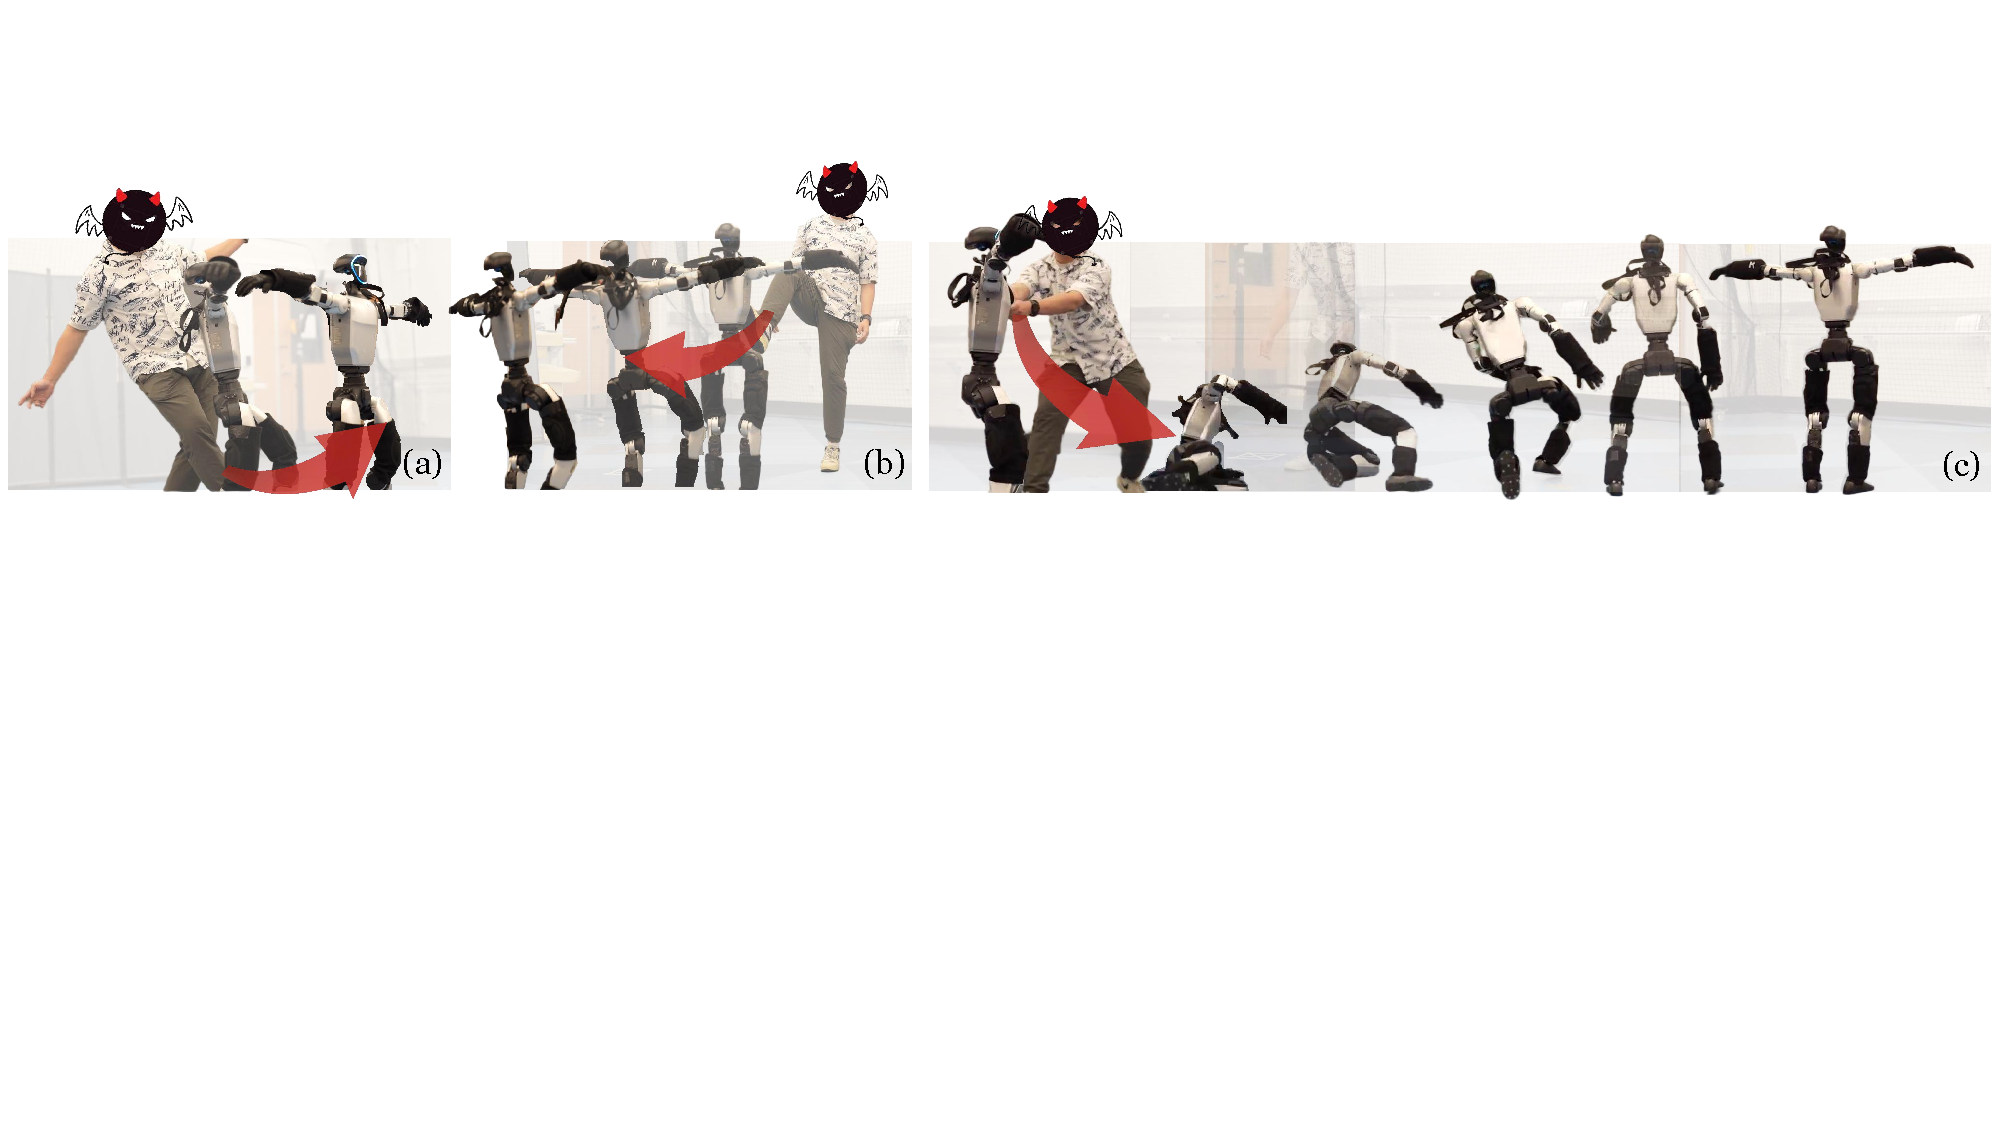
\includegraphics[width=\linewidth]{image/disturbance_rejection_1.pdf}
    \caption{\small Disturbance Rejection: (a) Keeps steady when kicked in the leg. (b) Absorbs a hard push with one smooth rear step. (c) \emph{Naturally} stands up and returns to T-pose after being yanked down.}
    \label{fig:disturbance}
\end{figure}
% One notable advantage of this policy is its compliance and robustness. As shown in Figure~\ref{fig:disturbance}, ~\ref{figure_2_teaser}, powered by our framework, the robot can react to strong disturbances such as fierce pushing, kicking, or being dragged to the ground in a human-like manner. After a strong forward push, it instinctively closes its arms, takes several quick steps in a running-like pose, then gradually slows down and reopens its arms (shown in Figure~\ref{figure_1_teaser}). \yitang{i want to stress this "robustness" and say better than unitree robustness testing demo} Although only a single latent vector from the static t-pose is always input to the policy, the policy will automatically and naturally deviate from the reference t-pose, takes a running-pose for recovery, before go back to track the t-pose, like a humand would do.
\textbf{Disturbance Rejection.}
One notable advantage of our policy is its strong compliance and robustness. As illustrated in Fig.~\ref{figure_1_teaser} and ~\ref{fig:disturbance}, our framework enables the robot to withstand severe disturbances—such as fierce pushes, kicks, or even being dragged to the ground, while recovering in a natural, human-like manner. For example, after a strong forward push, the robot instinctively closes its arms, takes several rapid steps in a running-like pose, and then slowly slows down before reopening its arms (Fig.~\ref{figure_1_teaser}). This level of robustness goes beyond the typical demonstrations seen in previous works: rather than fiercely reacting to the disturbances, our policy autonomously adapts. Although it receives only a single latent z from the static T-pose as input, it can automatically deviate from the reference posture, adopt a dynamic recovery pose, and eventually return to tracking the original T-pose just as a human would.

\begin{figure}[t]
    \centering
    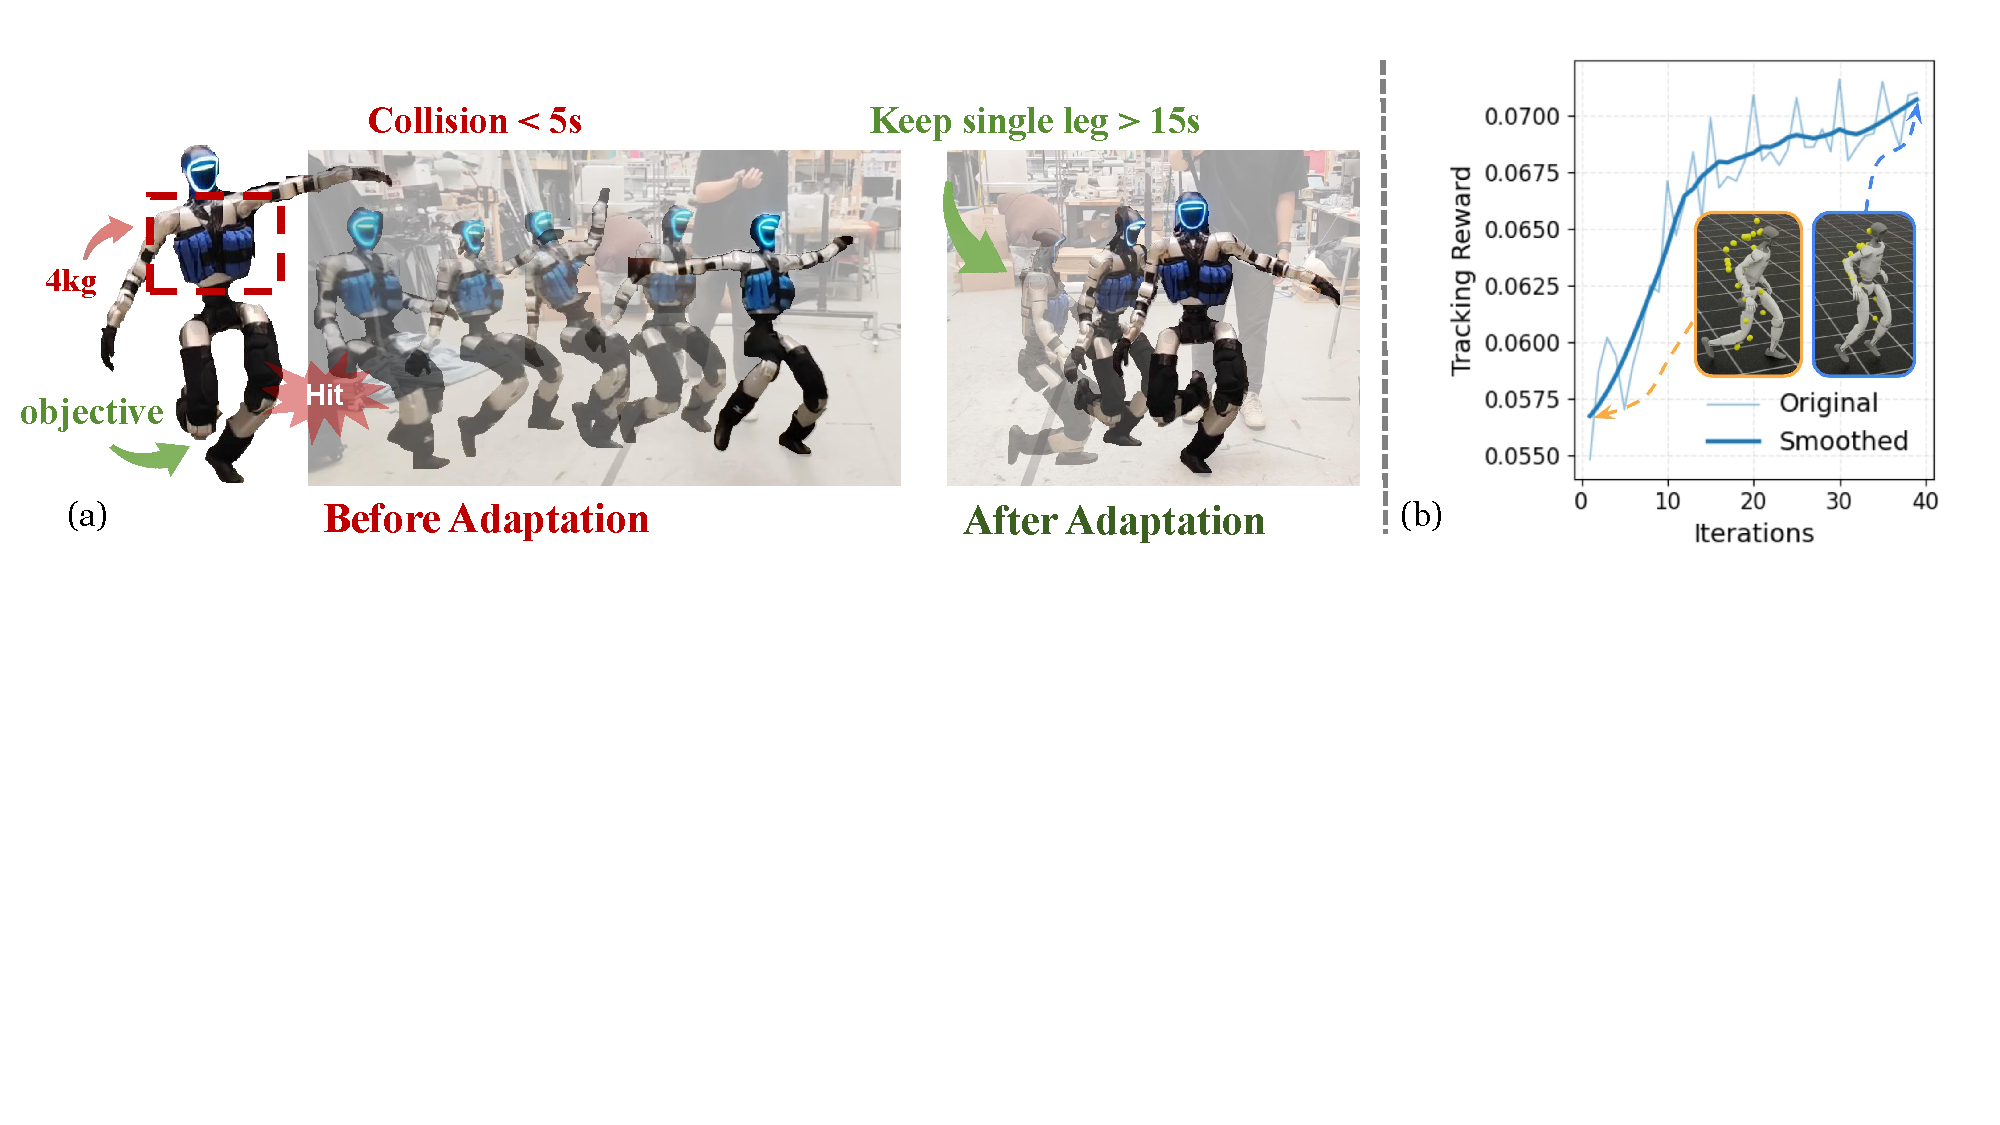
\includegraphics[width=.9\linewidth]{image/adaptation_final.pdf}
    \caption{Few-Shot Adaptation: (a) Single-pose adaptation improving single-leg standing under an additional payload. (b) Trajectory adaptation reduces tracking error.
}
    \label{fig:adaptation}
\end{figure}

\vspace{-0.3cm}

\subsection{Efficient Adaptation for \method{}}
\vspace{-2mm}
In this section we show how we leverage adaptation to improve the zero-shot inference performance under dynamics shift.
% \subsection{Visualizing the Latent Space of \method{}}

\textbf{Single Pose Adaptation.} We perform \emph{few-shot single-pose adaptation} in simulation to learn to stand on a single leg while carrying a payload. In simulation we increase the weight of the torso link by \textbf{4\,Kg}. Starting from the zero-shot latent $z^{\text{init}}$, we apply $20$ iterations of CEM to obtain $z^{\star}$, augmenting the rollout objective with a sparse task term $r\;=\;\mathbf{1}_{\{\,h_{\text{right foot}}>0.15~\mathrm{m}\ \wedge\ \text{no-contact}\,\}}$, 
which encourages right-foot clearance while avoiding unintended contacts. We deploy $z^\star$ on the real robot with a 4\,Kg mass rigidly attached to the torso.
As shown in~\Cref{fig:adaptation}\,(a), without adaptation, the motion driven by $z^{\text{init}}$ destabilizes and produces an environmental collision within $5\,\mathrm{s}$. In contrast, the optimized prompt $z^{\star}$ maintains single-leg balance for over $15\,\mathrm{s}$. These results indicate that prompt-level optimization alone can compensate for the payload-induced dynamics shift, without fine-tuning the model parameters.

\textbf{Trajectory Adaptation.}
For trajectory adaptation, we focus on optimizing a leaping motion under altered ground friction. We perform dual-annealing trajectory optimization \citep{xue2025full} in simulation using the explicit tracking reward defined in \citep{Luo2023phc}. We used sampling with particle count $N = 2048$, temperature schedules $\beta_{1} = 0.85$ and $\beta_{2} = 0.9$, and optimization iterations $M = 6$. The reward curve and before/after adaptation key-point tracking performance is shown in Fig.~\ref{fig:adaptation}(b), showing that our method significantly improves tracking accuracy, reducing error by $\sim$\emph{29.1}\%.

\subsection{The Latent Space Structure of \method{}}
\label{sec:latent}
\vspace{-2mm}
% \tonghe{This section may need another name? coz we also talk about interpolation.}\\
% \tonghe{
% Contact Tonghe for any questions in this part. 
% }\\
As mentioned in Sect.~\ref{sec:prelim}, \method{} provides an \textbf{interpretable} and \textbf{structured} representation of the behaviors of a humanoid robot. This representation not only facilitates understanding of the policy space but also enables instantaneous interpolation of existing skills without retraining. 

% \vspace{-2mm}
\textbf{Visualizing the Latent Space.}
 To examine the structure of the latent space, we sample latent vector trajectories and project them onto a two-dimensional plane (Fig.~\ref{fig:latent_z_map_2d}) to visualize the space, and also use a three-dimensional sphere to present representative latent generated for \emph{tracking, reward optimization and goal reaching}(Fig.~\ref{fig:latent_z_map_3d}) using t-SNE~\citep{tsne}. We can see the latent space is organized by motion style: semantically similar trajectories cluster, revealing a shared task centric structure.

% \begin{figure}[h]
%     \centering
%     \includegraphics[width=0.8\textwidth]{image/All-Tasks__tsne_3d_cropped.pdf}
%     \caption{t-SNE visualization of representative motions in 3D sphere.}
%     \label{fig:latent_z_map}
% \end{figure}
% \begin{figure}[h]
%     \centering
%     \includegraphics[width=0.8\textwidth]{image/All-Tasks_ts.pdf}
%     \caption{t-SNE visualization of representative motions in 2D plane.}
%     \label{fig:latent_z_map}
% \end{figure}

\begin{figure}[t]
    \centering
    \begin{subfigure}{0.3\textwidth}
        \centering
        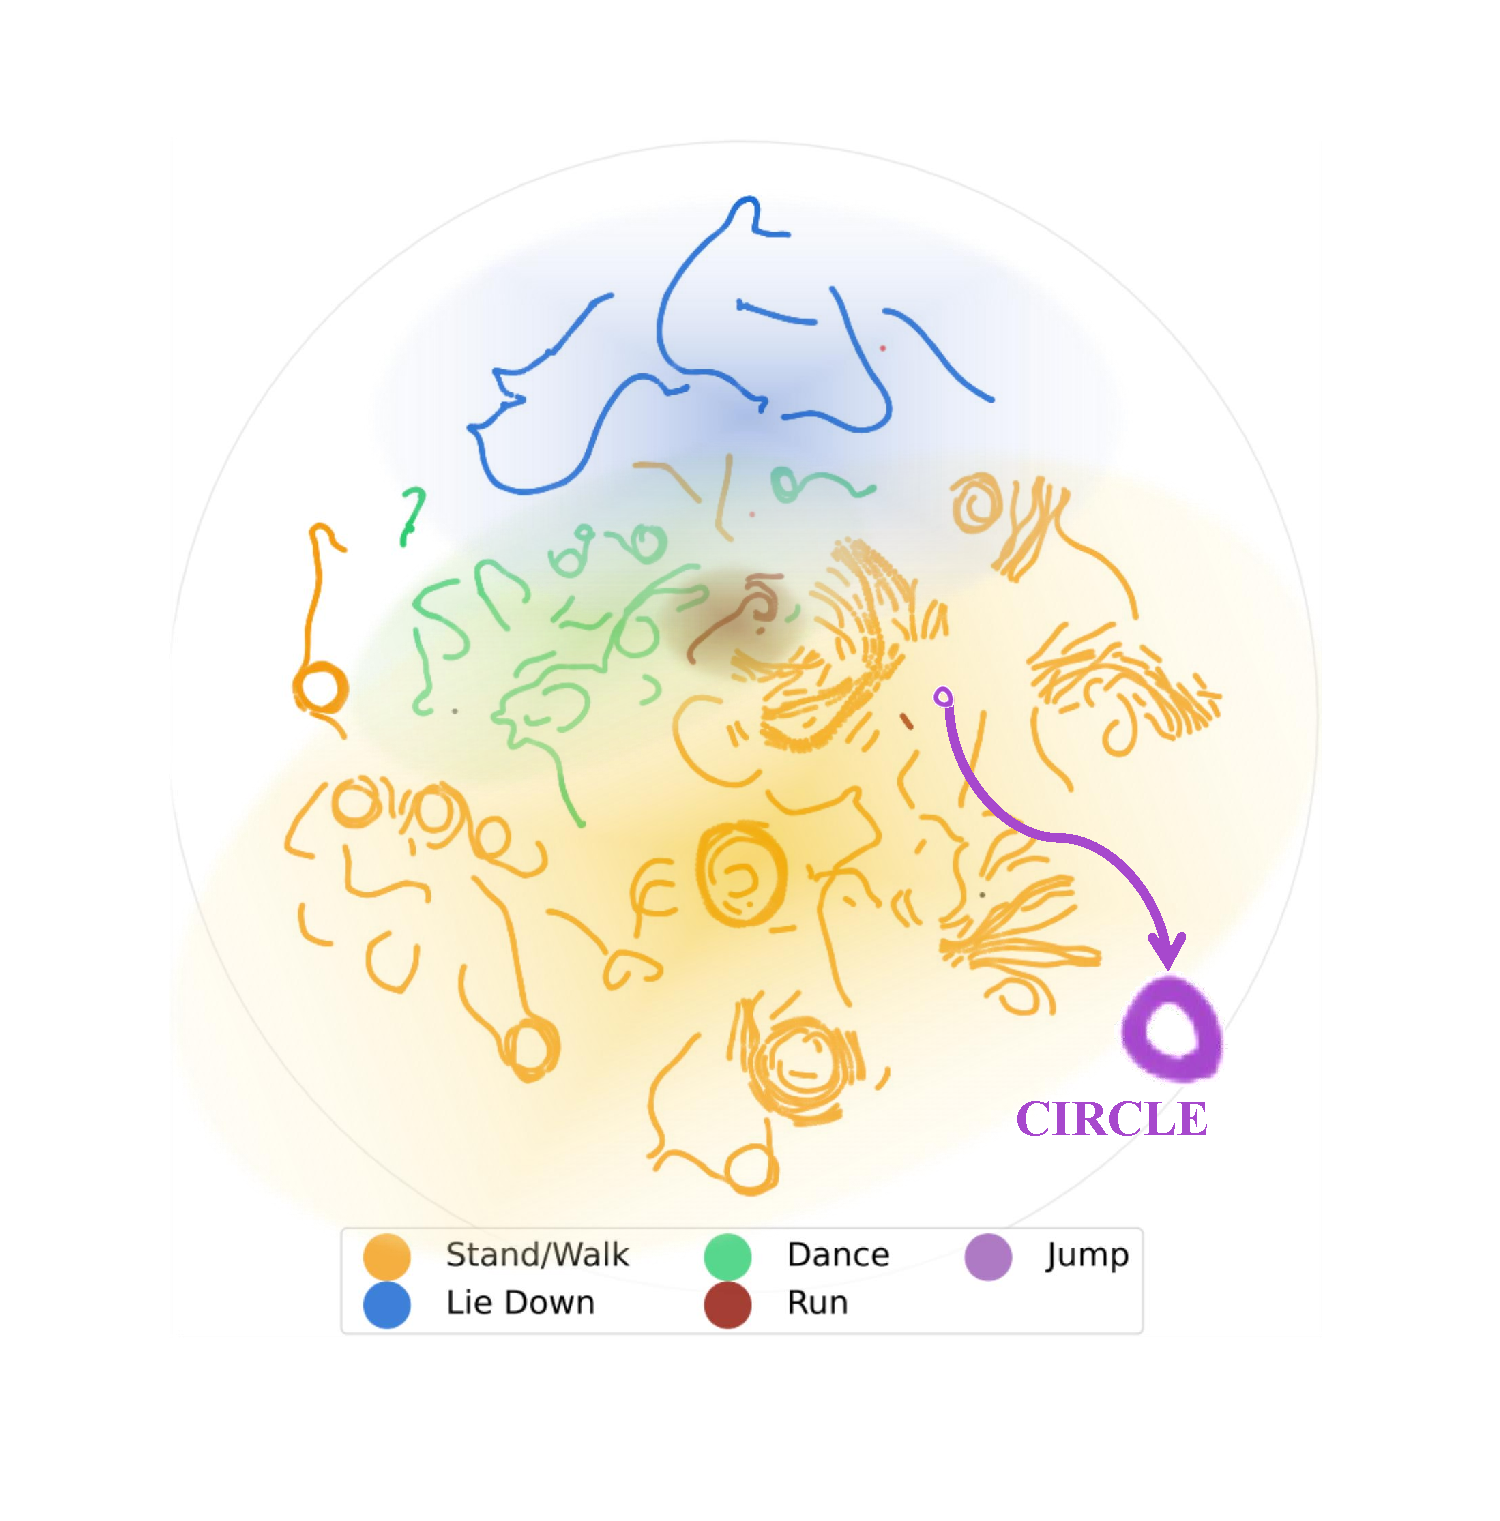
\includegraphics[width=.85\textwidth]{image/2d-tsne.pdf}
        \caption{Tracking trajectories segment the latent space (2D).}
        \label{fig:latent_z_map_2d}
    \end{subfigure}
      % \hfill
    \begin{subfigure}{0.32\textwidth}
        \centering
        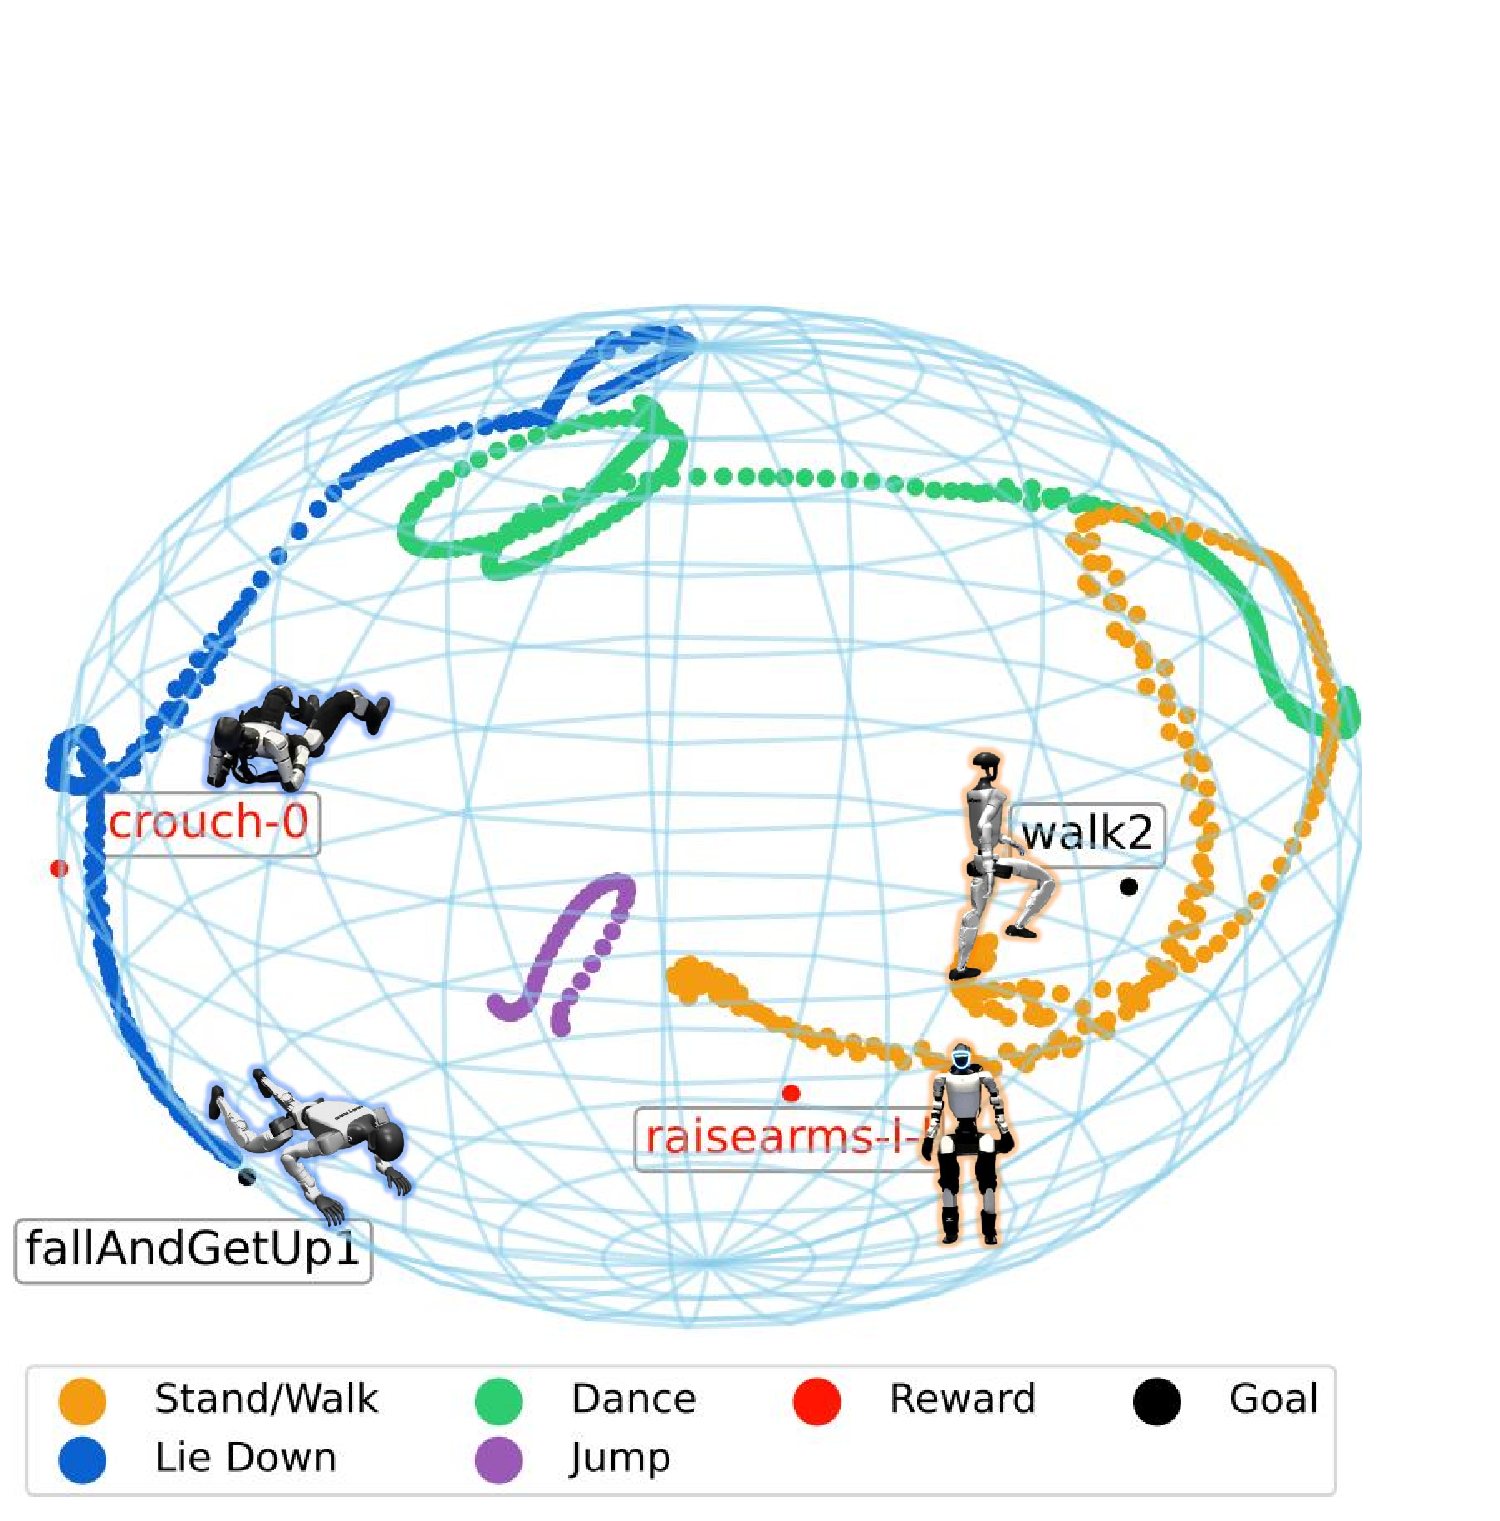
\includegraphics[width=.9\textwidth]{image/3d-tsne.pdf}
        \caption{Representative latents (3D).}
        \label{fig:latent_z_map_3d}
    \end{subfigure}
    \label{latent_z_map}
    \begin{subfigure}{0.28\textwidth}
        \centering
        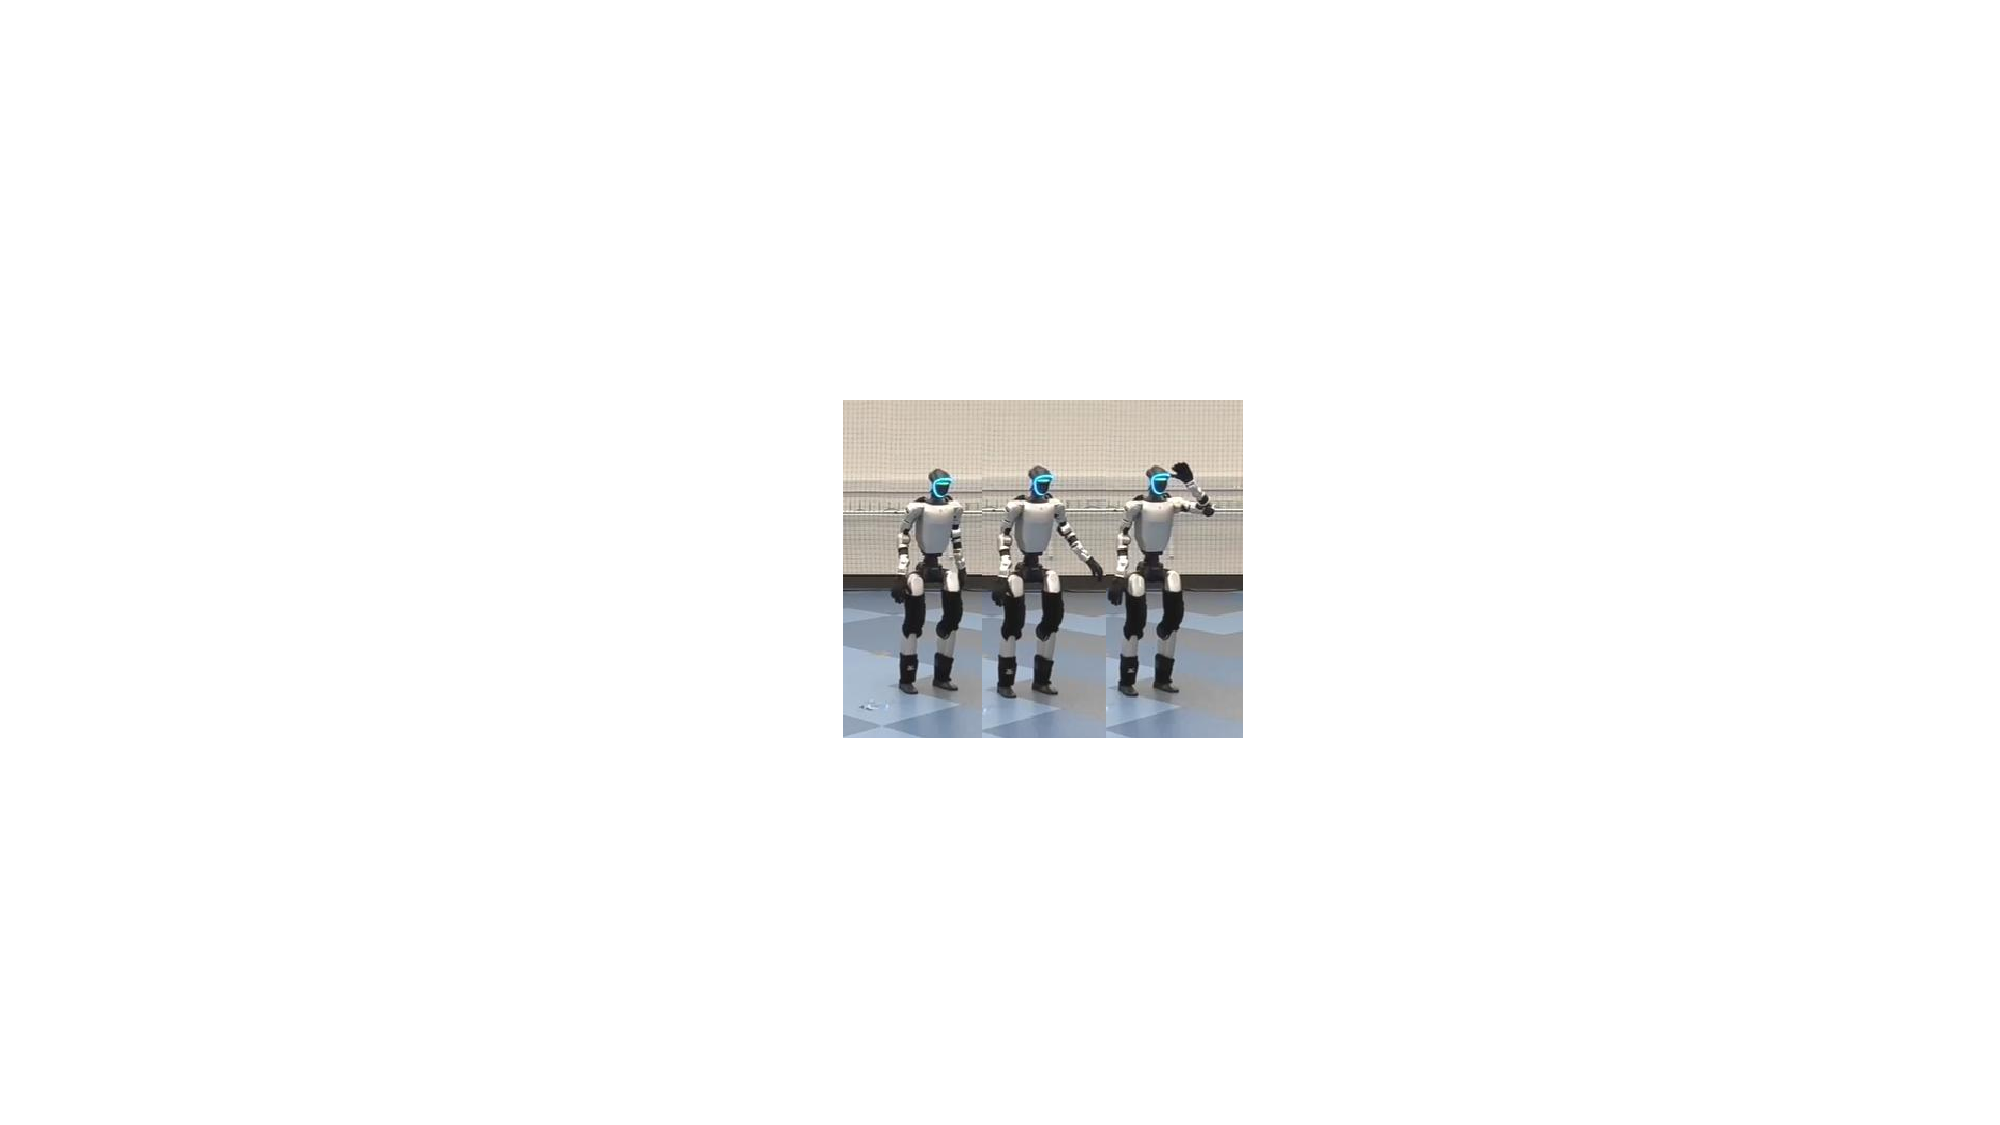
\includegraphics[width=\textwidth]{image/interpolation_final.pdf}
        \caption{Interpolation visualization}
        \label{fig:interpolation}
    \end{subfigure}
        \caption{Latent space visualization and analysis.}
\end{figure}
% \vspace{-2mm}
\textbf{Motion Interpolation on the Latent Space.}
The structured nature of $\mathcal{Z}$ enables smooth interpolation between latent representations. We can leverage Spherical Linear Interpolation~\citep{slerp} to generate intermediate latent vectors along the geodesic arc between the two end-points. To evaluate interpolated behaviors, we feed the resulting in-between $z_{t=0.5}$ into the \method{} policy, and deploy it on both simulated and real humanoid robots. As shown in Fig.~\ref{fig:interpolation}, the interpolated policy produces \emph{semantically meaningful} intermediate skills in a \emph{zero-shot} manner. These behaviors compose immediately—\emph{no additional training} required.

% The exact form of the interpolated points is specified by
% \begin{equation}
% \begin{aligned}
% z_{t} := \frac{\sin((1-t)\theta)}{\sin \theta}z_0 + \frac{\sin(t\theta)}{\sin \theta}z_1,
% \quad \theta := \arccos\left(\langle z_0, z_1 \rangle\right), \ z_0\ne z_1. 
% \end{aligned}
% \end{equation}
% for any interpolation parameter $t\in[0,1]$. 





